
%(BEGIN_QUESTION)
% Copyright 2007, Tony R. Kuphaldt, released under the Creative Commons Attribution License (v 1.0)
% This means you may do almost anything with this work of mine, so long as you give me proper credit

The tension in the cable holding up the sign is . . .

$$\includegraphics[width=15.5cm]{i02753x01.eps}$$

\begin{itemize}
\item{(A)} less than the weight of the sign
\vskip 5pt 
\item{(B)} always changing with temperature
\vskip 5pt 
\item{(C)} equal to the weight of the sign
\vskip 5pt 
\item{(D)} greater than the weight of the sign
\vskip 5pt 
\item{(E)} a negative quantity
\end{itemize}

\underbar{file i02753}
%(END_QUESTION)





%(BEGIN_ANSWER)

{\bf (D)} greater than the weight of the sign
 
%(END_ANSWER)





%(BEGIN_NOTES)


%INDEX% Certification exam: chemistry and physics

%(END_NOTES)


